
\section{Problem Definition and System Overview}

\subsection{Problem Definition}
This paper addresses aerial object navigation, a variant of the ObjectNav~\cite{batra2020objectnav} task adapted for aerial agents in large-scale outdoor environments. The agent must explore an unknown environment to locate an open-set target object specified by a natural language instruction, while minimizing path length. Task success is achieved when the agent reaches within a predefined distance of the target and executes a stop action.


\subsection{Asynchronous System Architecture}
The system architecture of \sysname is illustrated in \fig\ref{fig:sysoverview}(a). Current practices typically use high-latency VLMs to output step-wise sparse actions, which either induce a stop-and-infer loop or yield temporally mismatched actions, as shown in \fig\ref{fig:sysoverview}(b).
In contrast, \sysname introduces a \textit{Dual-pathway Asynchronous} architecture that establishes a principled interface between VLM reasoning and path planning. 
The core idea is to repurpose the VLM from a direct action generator to a dense semantic signal generator, producing language-conditioned, region-level semantic priors that provide spatially dense guidance.
The VLM and the planner operate at their native frequencies without mutual blocking, with their synergy mediated by a shared intermediate 3D representation (\ie, 3D value map). 
Specifically, the VLM-driven reasoning pathway runs at low frequency to infer these priors from selected observations and asynchronously integrates them into the shared representation. 
Concurrently, the high-frequency planning pathway continuously generates trajectories from the evolving representation, jointly leveraging its semantic priors and geometric information without synchronizing with VLM inference. 
By integrating semantic evidence over time, the shared representation reconciles potential contradictions in VLM outputs and mitigates VLM's limited 3D scene understanding, enabling continuous long-horizon flight with dense semantic guidance rather than fragmented motion driven by sparse, delayed actions.


From the algorithm perspective, \sysname comprises two core modules: the Active Dual-Task Reasoning (ADTR) (\S\ref{IV}) and the Semantic-Geometric Coherent Planning (SGCP) (\S\ref{V}).
ADTR selects informative keyframes and prompts VLM for two tasks: (\textit{i}) infer semantic values across diverse regions to update a 3D value map for exploration guidance; and (\textit{ii}) verify whether detected objects match the task instruction.
Based on the 3D value map, SGCP achieves spatially consistent planning by strategically balancing semantic guidance with geometric travel efficiency.
It first clusters frontiers based on semantic similarity and geometric proximity, then generates viewpoints that prioritize observing high-value regions. Finally, it computes a globally optimal tour that prioritizes semantically valuable regions while minimizing travel distance.


\sysname operates in three stages: (\textit{i}) Initialize: the drone initializes by rotating 360° in place to observe the surroundings; (\textit{ii}) Search: after initialization, the ADTR module continuously updates 3D value maps to guide the SGCP module in generating exploration trajectories; (\textit{iii}) Navigate to target: upon target confirmation by the ADTR module, the system transitions to goal-directed navigation and terminates once the drone reaches sufficient proximity to the target.


\section{Active Dual-Task Reasoning}\label{IV}
VLMs pretrained on large amounts of image-text datasets have internalized extensive commonsense knowledge. However, transferring this semantic understanding to continuous 3D space for navigation remains challenging. This challenge is compounded by the fact that drone-mounted cameras generate high-frequency image streams ($>$20 Hz) with substantial redundancy, making exhaustive per-frame VLM processing computationally prohibitive ($>$2000 ms latency per query).

To address these issues, we propose a Active Dual-Task Reasoning (ADTR) module, as illustrated in \fig\ref{fig:module1}. We ground our design on two key observations: 
(\textit{i}) VLMs can directly quantify the semantic relevance of image regions as probabilities conditioned on free-form instructions, providing a quantitative way to identify high-value regions in the drone's planning space; (\textit{ii}) Task-relevant semantic information (i.e., critical objects and cues) in outdoor scenes exhibits high sparsity, which allows for substantial filtering of redundant frames while preserving critical information. We describe the details in the following sections.


\subsection{Active Keyframe Construction}\label{IVA}
To address the computational burden of processing high-frequency image streams from the drone-mounted camera, we adaptively select observed images to construct two types of keyframes: coverage-aware keyframes to maximize geometric coverage of the exploration space, and task-aware keyframes to capture fine-grained and task-relevant information.

\subsubsection{Coverage-aware Keyframe Construction}
We first introduce coverage-aware keyframes to ensure comprehensive geometric coverage of the exploration space. To achieve this, we quantify spatial coverage by discretizing the environment into a 3D voxel grid with resolution $r$. Consider the sequential observations $\mathcal{I} = \{I_1, I_2, \ldots, I_N\}$ from the drone's onboard camera, where each observation $I_i$ consists of an RGB image and its corresponding camera pose. A coverage-aware keyframe is then defined as $\mathcal{K}_s^i = \langle I_i, \mathcal{V}(I_i) \rangle$, where $I_i$ is the observation and $\mathcal{V}(I_i) \subset \mathbb{R}^3$ is the set of 3D voxels visible from the camera pose. The coverage-aware keyframe set at time $t$ is denoted as $\mathcal{S}_t^{\text{cov}}$.

To maximize geometric coverage while minimizing redundancy, we employ a voxel-based overlap criterion. 
Given the current observation $I_t$ and a keyframe $\mathcal{K}_s^i = \langle I_i, \mathcal{V}(I_i) \rangle \in \mathcal{S}_{t-1}^{\text{cov}}$, the overlap ratio between $I_t$ and $I_i$ is defined as $\mathcal{R}(I_t, I_i) = |\mathcal{V}(I_t) \cap \mathcal{V}(I_i)| / |\mathcal{V}(I_t)|$,
where $|\cdot|$ denotes set cardinality. 
For each new observation $I_t$ at time $t$, it is added to the keyframe set if its overlap with all existing keyframes remains below threshold $\tau_{\text{cov}}$, which can be expressed as
\begin{equation}
\mathcal{S}_t^{\text{cov}} = \mathcal{S}_{t-1}^{\text{cov}} \cup \{\langle I_t, \mathcal{V}(I_t) \rangle\}, \ \text{if } \mathcal{R}(I_t, I_i) < \tau_{\text{cov}}, \forall \mathcal{K}_s^i \in \mathcal{S}_{t-1}^{\text{cov}}.
\end{equation}
This criterion ensures that only observations providing sufficient novel geometric coverage are retained, thereby maintaining a compact yet comprehensive representation of the explored space.

\subsubsection{Task-aware Keyframe Construction}
While coverage-aware keyframes ensure comprehensive spatial exploration, they do not guarantee semantic richness relevant to the target object. We therefore introduce task-aware keyframes that are constructed to contain foreground object-level details and contextual scene-level cues pertinent to the instruction, providing the VLM with informative content necessary for accurate target verification.

Specifically, a task-aware keyframe $\mathcal{K}_e^j = \langle I_j, \mathcal{O}(I_j) \rangle$ encodes object-centric scene understanding, where $\mathcal{O}(I_j) = \{o_1, o_2, \ldots, o_M\}$ represents the set of objects detected in observation $I_j$. Each object $o_j$ is characterized by a tuple $(c_j, s_j, \mathbf{x}_j)$, consisting of object category $c_j$, detection confidence score $s_j \in [0,1]$, and 3D position $\mathbf{x}_j \in \mathbb{R}^3$ obtained through object detection, segmentation, and coordinate transformation~\cite{gu2024conceptgraphs}. 
Similarly, we maintain a task-aware keyframe set $\mathcal{S}_t^{\text{task}}$.
Given a natural language instruction $\mathcal{L}$ (\eg, ``find a trash bin on the roadside''), we first query a VLM to identify the top-$K$ object categories $\mathcal{C}_{\text{target}} = \{c_1^*, c_2^*, \ldots, c_K^*\}$ most relevant to the task. For each observation $I_t$, we extract its detected object categories $\mathcal{C}(I_t) = \{c_j \mid o_j \in \mathcal{O}(I_t)\}$. The observation is promoted to a task-aware keyframe if it contains at least one target-relevant object:
\begin{equation}
    \mathcal{S}_t^{\text{task}} = \mathcal{S}_{t-1}^{\text{task}} \cup \{\langle I_t, \mathcal{O}(I_t) \rangle\}, \quad \text{if } \mathcal{C}(I_t) \cap \mathcal{C}_{\text{target}} \neq \emptyset.
\end{equation}
This filtering mechanism discards semantically irrelevant observations while preserving all task-critical visual information for VLM reasoning.

\begin{figure*}[t]
    \centering
    \setlength{\abovecaptionskip}{-3pt}  % 默认约为 10pt
    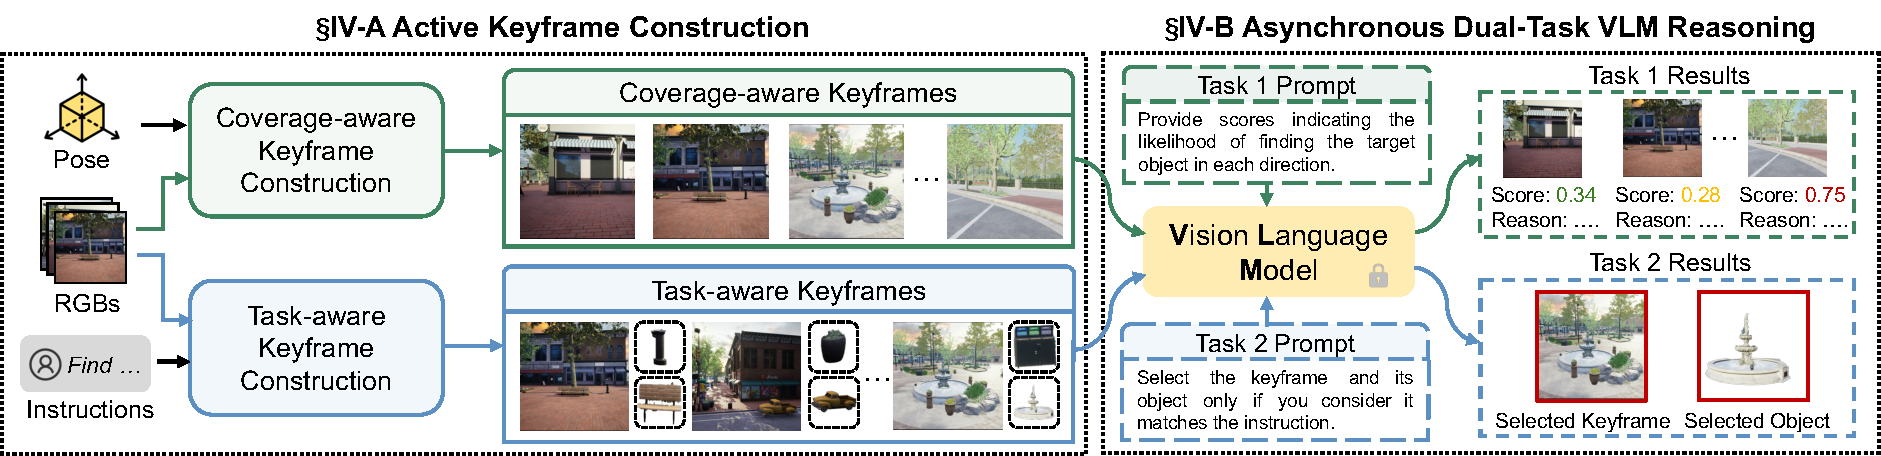
\includegraphics[width=0.98\linewidth]{figures/SSR-2.pdf}
    \caption{Illustrations of the Active Keyframe Construction and Asynchronous Dual-Task VLM Reasoning Modules. ADTR constructs a coverage-aware keyframe set and a task-aware keyframe set, then queries the VLM for semantic value inference (Task 1) and related object verification (Task 2), respectively.}
    \label{fig:module1}
    \vspace{-10pt}
\end{figure*}
\subsection{Asynchronous Dual-Task VLM Reasoning}\label{IV-B}
The constructed keyframes are fed to our dual-task VLM reasoning module for 
semantic value inference and object verification. To mitigate the variable and potentially long inference latency of VLM queries (sometimes up to 10s under network instability), both tasks execute asynchronously. The VLM reasoning is triggered when either keyframe set reaches its capacity threshold, after which the sets are reset to accumulate new keyframes for the next reasoning cycle.

\subsubsection{Task 1: Semantic Value Inference} 
Due to the high latency of VLM inference, generating per-step action commands from the VLM is impractical for real-time flight. Instead, we use the VLM to reason region-level target-presence probabilities for the scenes captured in keyframes. This probabilistic signal serves as a semantic prior, offering more informative guidance for subsequent motion generation.
Specifically, given the instruction $\mathcal{L}$ and the coverage-aware keyframe set $\mathcal{S}_t^{cov}$, we prompt the VLM to assign a semantic value $v_i \in [0,1]$ to each keyframe $\mathcal{K}_s^i \in \mathcal{S}_t^{cov}$:
\begin{equation}
    v_i = \text{VLM}(\mathcal{K}_s^i, \mathcal{L}),
\end{equation}
where $v_i$ quantifies the probability that the region represented by $\mathcal{K}_s^i$ contains the target object described in $\mathcal{L}$. For instance, given the instruction ``find the white football on the grass'', the VLM assigns higher semantic values to keyframes depicting grassy areas and lower values to keyframes showing basketball courts or buildings. 

\subsubsection{Task 2: Related Object Verification}
Open-vocabulary detectors often produce erroneous labels when objects are occluded, distant, or visually ambiguous. Moreover, they lack contextual understanding to distinguish semantically similar objects (\eg, identifying a black trash bin among bins of different colors). Therefore, we employ the VLM to verify and identify the correct target object from detection candidates based on the given instruction.

Given the task-aware keyframe set $\mathcal{S}_t^{task}$ and instruction $\mathcal{L}$, the VLM selects the target object through:
\begin{equation}
    (\mathcal{K}_e^*, o^*) = \text{VLM}(\mathcal{S}_t^{task}, \mathcal{L}),
\end{equation}
\noindent where $\mathcal{K}_e^*$ denotes the selected keyframe containing the target object, and $o^* \in \mathcal{O}(\mathcal{K}_e^*)$ represents the identified target object from the detection candidates. By integrating both visual appearance cues and spatial context such as object relationships, relative positions, and background information, the VLM performs instruction-specified reasoning to accurately identify the target object.


\subsection{3D Value Map Composition}\label{IV-C}
To guide the drone's search in 3D space, we maintain a 3D value map that encodes the target-presence potential across the search environment based on the semantic values obtained from Task 1. These values are projected into the 3D scene according to the camera's field of view, with occluded regions excluded. A higher value in a region indicates a stronger probability that the target object is located there. By accumulating language-conditioned evidence from multiple viewpoints, the map consolidates potentially inconsistent VLM outputs into a single spatial belief, yielding a more coherent target-probability field for downstream planning and mitigating the VLM’s limited 3D scene understanding.
\subsubsection{Map Representation}
We define a 3D value map $\mathbf{V} \in \mathbb{R}^{W \times H \times D}$ discretized with voxel resolution $r$, comprising two channels: $\mathbf{V} = (\mathbf{V}^{sem}, \mathbf{V}^{conf})$, where $\mathbf{V}^{sem} \in [0,1]$ encodes target-finding potential and $\mathbf{V}^{conf} \in [0,1]$ represents estimation confidence.
For each voxel $\mathbf{v}_k$ at position $\mathbf{x}_k$ visible from drone pose $\mathbf{p}_t$ at distance $d_k = \|\mathbf{x}_k - \mathbf{p}_t\|_2$, the confidence is computed as:
$c_k^t = \max\left(0, 1 - \frac{d_k}{d_{max}}\right)$, where $d_{max}$ is the maximum sensing range. This formulation ensures that confidence decreases with observation distance, reflecting the degradation in visual information quality.

\subsubsection{Map Fusion}
To enable continuous navigation guidance, the value map is updated \textit{asynchronously} as soon as semantic values are returned from Task 1.
Specifically, when the semantic value $v_i$ for keyframe $\mathcal{K}_s^i$ is returned at time $t$, voxels in $\mathcal{V}(I_i)$ are updated via confidence-weighted aggregation~\cite{yokoyama2024vlfm}:
\begin{equation}
    v_k^t = \frac{c_k^{t-1} \cdot v_k^{t-1} + c_k^t \cdot v_i}{c_k^{t-1} + c_k^t},
\end{equation}
where $v_k^{t-1}$ and $c_k^{t-1}$ denote previous values. The confidence is updated to emphasize higher-confidence observations: $c_k^t = \frac{(c_k^{t-1})^2 + (c_k^t)^2}{c_k^{t-1} + c_k^t}$.
This scheme integrates multi-viewpoint information with confidence-based weighting, yielding an effective intermediate representation layer for path planning.


\section{Semantic-Geometric Coherent Planning}\label{V}
% \section{Semantic-informed Consistent Planning}\label{V}
Given the 3D value map, planning efficient search trajectories remains significantly challenging due to the inherent conflict between semantic ambiguity and geometric determinism. Unlike dense geometric maps, VLM-derived semantic priors are sparse, probabilistic, and spatially diffuse. Strictly prioritizing high-value regions often triggers oscillatory motion when multiple candidate regions exhibit comparable semantic values, resulting in inefficient circuitous routes. Conversely, prioritizing geometric proximity degrades the system into a blind explorer that delays visiting target-relevant regions. Existing 
approaches lack a principled mechanism to dynamically reconcile these heterogeneous information sources (i.e., semantic and geometric), leading to myopic search behaviors that impair overall search efficiency.


To tackle this challenge, we propose a hierarchical Semantic-Geometric Coherent Planning (SGCP) algorithm that systematically balances semantic guidance with geometric travel efficiency across planning stages. First, we introduce a semantic frontier structure that clusters frontier voxels by both semantic similarity and spatial proximity, enabling fine-grained task-aware exploration beyond purely geometric approaches. Second, we design semantic-geometric viewpoint generation that maximizes information gain weighted by semantic values, ensuring each viewpoint prioritizes target-relevant regions. Third, we develop adaptive constraint-injected global planning that enforces semantic priorities through selective precedence constraints while preserving geometric optimization flexibility, providing flexible search behavior that adapts to diverse environments. This unified design coherently integrates semantic guidance and geometric motion efficiency at frontier, viewpoint, and tour levels, achieving spatially consistent search trajectories with minimal redundant coverage.


\subsection{Semantic-aware Frontier Construction}\label{V-A}
Frontiers are defined as boundary regions between known free space and unknown space~\cite{yamauchi1997frontier}. 
Traditional frontier-based exploration methods leverage this structure to achieve complete scene coverage through purely geometric distance metrics, without considering task relevance~\cite{zhang2024falcon}. 
In contrast, we introduce the semantic frontier that seamlessly integrates geometric information with semantic cues, enabling downstream planners to efficiently explore scenes with fine-grained open-set semantic understanding.

\subsubsection{Semantic Frontier Formulation}
We utilize a volumetric occupancy grid map to represent the environment~\cite{han2019fiesta}, where each frontier voxel $k$ is assigned a semantic value $v_k \in [0,1]$ based on its coordinates in the 3D value map.
A \textit{semantic frontier cluster} is formally defined as $F_i = \langle \mathcal{C}_i, \mathbf{p}_i, s_i \rangle$, where:
\begin{itemize}
    \item $\mathcal{C}_i = \{c_1, c_2, \ldots, c_{n_i}\}$ denotes the set of frontier voxels belonging to cluster $i$,
    \item $\mathbf{p}_i \in \mathbb{R}^3$ represents the geometric centroid of $\mathcal{C}_i$,
    \item $s_i = \frac{1}{|\mathcal{C}_i|}\sum_{c_j \in \mathcal{C}_i} v(c_j)$ indicates the average semantic value of the cluster $i$ and $v(c_j)$ denotes the semantic value of voxel $c_j$.
\end{itemize}


\subsubsection{Incremental Frontier Update}
Each time the occupancy grid map is updated by new sensor measurements, we perform an incremental update of the frontier structure to maintain computational efficiency. We first remove frontier clusters that are affected by the newly observed regions~\cite{zhou2021fuel}. To identify new frontiers, we design a semantic-constrained region growing algorithm.

Specifically, we initiate the region growing process from seed voxels $c_s$ located at the interface between known free space and unknown regions. The algorithm performs breadth-first expansion to aggregate spatially connected frontier cells into clusters~\cite{mehnert1997improved}. Our key innovation is the incorporation of semantic constraints during this process.
Formally, let $\mathcal{N}(c)$ denote the set of spatially adjacent voxels to voxel $c$ in the 6-connected grid. During the expansion of cluster $F_i$ with seed voxel $c_s$, a neighboring voxel $c_j \in \mathcal{N}(c_k)$, where $c_k \in \mathcal{C}_i$, is added to the cluster if it satisfies:
\begin{equation}
    |v(c_j) - v(c_s)| < \tau_s \quad \text{and} \quad c_j \in \mathcal{U},
\end{equation}
where $\tau_s$ is a predefined semantic similarity threshold and $\mathcal{U}$ denotes the set of unvisited frontier voxels. 
Excessively large frontier clusters are then recursively split following~\cite{zhou2021fuel}.
This semantic-constrained expansion enables clustering of frontiers based on both semantic similarity and geometric proximity, thereby facilitating task-informed planning strategies.


\begin{figure}[t]
    \centering
    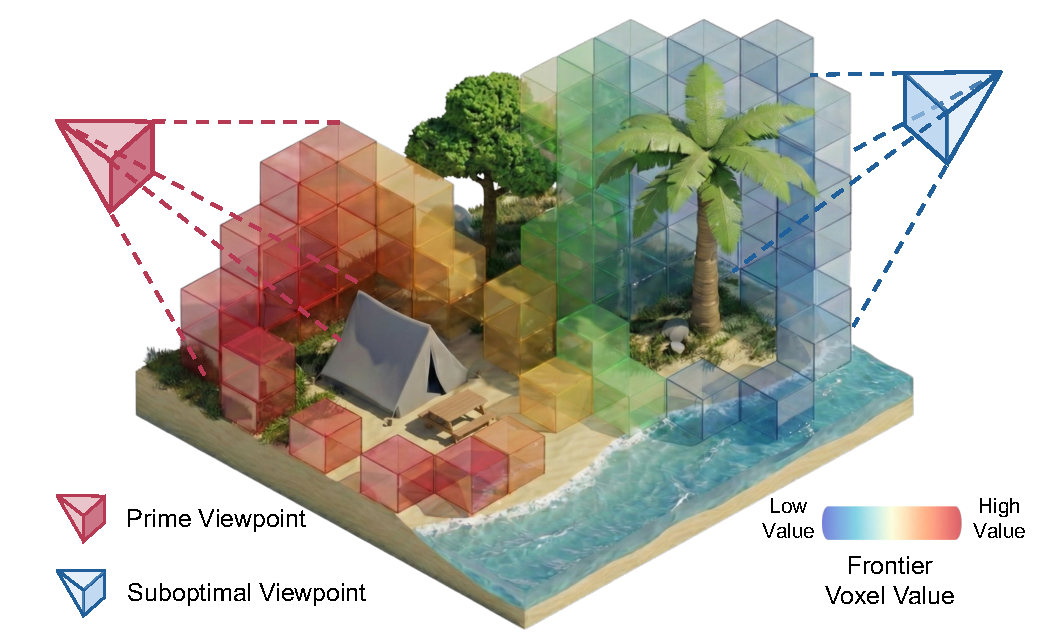
\includegraphics[width=0.95\linewidth]{figures/vp_gen.pdf}
    \caption{Illustration of Semantic-Geometric Viewpoint Generation. Given the instruction ``Fly to the tent on the beach'', frontier voxels near the target are assigned higher semantic values (red). The \textit{prime viewpoint} is selected to maximize information gain, computed as the sum of semantic values over observable frontier voxels, thereby focusing on the target tent.
 }
    \label{fig:module2-1}
    \vspace{-12pt}
\end{figure}

\subsection{Semantic-Geometric Viewpoint Generation}\label{V-B}
For each frontier cluster $F_i$, we generate a set of candidate viewpoints around the cluster's centroid $\mathbf{p}_i$ to enable observation of the unexplored regions~\cite{zhou2023racer}.
This yields a viewpoint set $\mathcal{U}_i = \{u_i^1, u_i^2, \ldots, u_i^{M_i}\}$, where each viewpoint $u_i^j = (\mathbf{p}_i^j, \theta_i^j)$ consists of position $\mathbf{p}_i^j$ and yaw angle $\theta_i^j$.

To select the most informative viewpoint for each cluster, we evaluate each candidate based on both geometric coverage and semantic importance, as illustrated in \fig\ref{fig:module2-1}. For each candidate viewpoint $u_i^j$, we first evaluate its coverage by identifying all frontier voxels within the sensor's field of view (FoV) that are not occluded by occupied voxels. We then quantify the information gain as the sum of semantic values over all observable voxels as $S(u_i^j) = \sum_{c_k \in \mathcal{N}_{obs}(u_i^j)} v(c_k),$
% \begin{equation}
%     S(u_i^j) = \sum_{c_k \in \mathcal{N}_{obs}(u_i^j)} v(c_k),
% \end{equation}
where $\mathcal{N}_{obs}(u_i^j)$ denotes the set of observable frontier voxels from viewpoint $u_i^j$.
The viewpoint with the highest information gain is selected as the \textit{prime viewpoint} $u_i^*$ for cluster $F_i$.
This approach ensures that the prime viewpoint not only maximizes the number of observable frontier voxels but also gives priority to voxels with higher semantic values, facilitating exploration of informative areas.


\begin{figure}[!t]
    \centering
    \setlength{\abovecaptionskip}{-3pt}  % 默认约为 10pt
    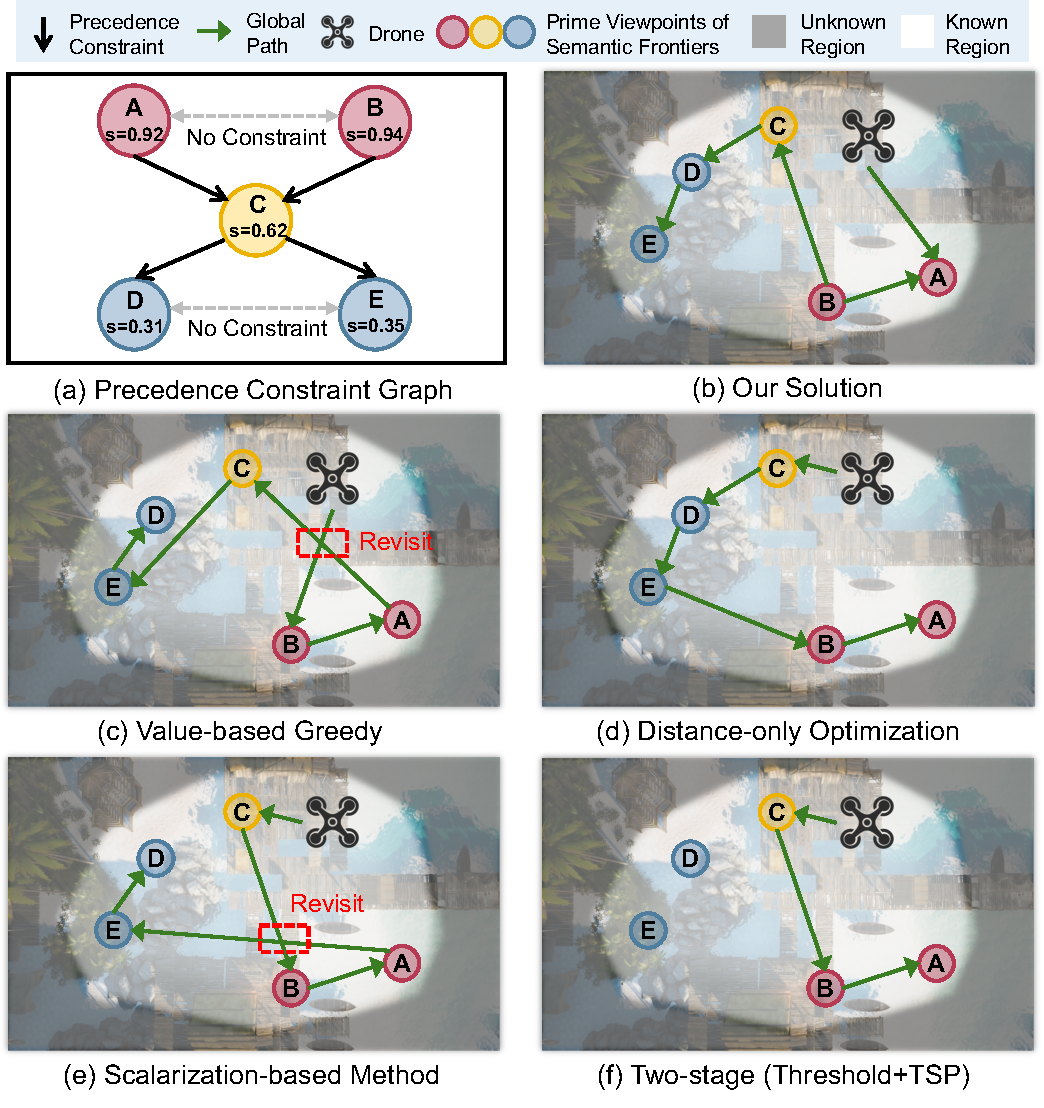
\includegraphics[width=0.98\linewidth]{figures/globalpath-5.pdf}
    \caption{
    Comparison of global planning strategies. (a) The constraint graph selectively enforces precedence only when semantic value differences are significant (e.g., A(0.92)$\rightarrow$C(0.62)), allowing geometric optimization for similar-value frontiers (e.g., A and B). (b) Our solution generates a globally coherent path that prioritizes high-value frontiers without revisits. (c)-(f) Baseline approaches tend to yield revisits of previously searched regions (red dashed boxes) or delay visits to semantically critical regions (A and B).
    }
    \label{fig:module2-2}
    \vspace{-12pt}
\end{figure}




% \subsection{Semantic-aware Global Path Planning}\label{V-C}
\subsection{Optimization with Selective Constraint Injection}\label{V-C}
Given a set of semantic frontier clusters, our objective is to compute a global exploration tour that prioritizes target-relevant regions while minimizing total traversal time. Existing planners typically optimize one side or combine both via heuristics, but neither yields consistently efficient tours. Value-based greedy selection (\fig\ref{fig:module2-2}(c)) ignores spatial structure and induces large detours when high-value frontiers are dispersed, whereas distance-only optimization (\fig\ref{fig:module2-2}(d)) prioritizes short moves and can defer semantically critical regions. Hybrid heuristics mainly adopt two paradigms. (\textit{i}) scalarization method greedily maximizes a utility score (e.g., value/distance), which tends to bias toward nearby moderate-value frontiers and postpone distant yet substantially higher-value regions (\fig\ref{fig:module2-2}(e)); (\textit{ii}) two-stage method thresholds semantic values to form a frontier subset and then solves a distance-optimal tour. This hard boundary may discard useful regions, and the distance-driven ordering within the subset does not preserve semantic priorities, providing no guarantee that higher-value regions are visited earlier (\fig\ref{fig:module2-2}(f)).


To address this challenge, our key idea is to \textit{selectively} inject ordering constraints only between frontier clusters whose semantic values differ significantly (\fig\ref{fig:module2-2}(a)), and the frontier visitation order is then optimized by minimizing the geometric traversal cost subject to these constraints. 
This design adapts naturally to the semantic value distribution: when a region is distinctly more target-relevant, dense precedence relations enforce early visitation; when semantic scores are comparable, the constraint set becomes sparse, allowing the visiting order to be dominated by geometric proximity. 
By reconciling semantics and geometry through a unified optimization framework with value-gap-derived precedence constraints, SGCP achieves semantic-driven exploration in scenarios with distinct high-value regions and geometry-efficient routing in semantically homogeneous ones, without requiring environment-specific parameter tuning.
This formulation can be transformed into a Sequential Ordering Problem (SOP)~\cite{hernadvolgyi2004solving}, which can be efficiently solved by off-the-shelf solvers. We provide the formal definition of the SOP and present our formulation and solution below.

\textit{Definition 1 (Sequential Ordering Problem)}:
Given a directed graph $G = (V, E)$, edge weight $w : E \to \mathbb{R}$ and a set of precedence constraints $\mathcal{P} \subseteq V \times V$, the SOP searches for a minimum cost permutation of vertices from $s \in V$ to $t \in V$ that satisfies the precedence constraints.


\subsubsection{Selective Precedence Constraint}
In our case, for each cluster $F_i$, we define a vertex $v_i \in V$ locates at its prime viewpoint $u_i^*$. 
We then enforce visiting priorities of high-value frontiers through precedence constraints that adapt to the semantic value distribution.
The precedence constraints set is defined based on semantic value differences:
\begin{equation}
    \mathcal{P} = \{(v_i,v_j) \mid s_i - s_j > \rho \},
\end{equation}
where $s_i$ is the semantic value of cluster $F_i$, and $\rho$ is a positive threshold controlling sensitivity to semantic differences. 
The precedence constraint $(v_i,v_j) \in \mathcal{P}$ enforces that the prime viewpoint $u_i^*$ of cluster $F_i$ (with higher semantic value) must be visited before the prime viewpoint $u_j^*$ of cluster $F_j$.
This design ensures that only semantically significant differences trigger ordering constraints (\fig\ref{fig:module2-2}(a)), allowing geometric optimization to dominate when semantic cues are weak.


\subsubsection{Geometric Cost Calculation}
While precedence constraints handle semantic priorities, geometric costs determine the actual traversal efficiency when semantic cues are weak.
For any two viewpoints $u_i = (\mathbf{p}_i, \theta_i)$ and $u_j = (\mathbf{p}_j, \theta_j)$, we define the geometric cost (\ie, edge weight $w$) as:
\begin{equation}
    C(u_i, u_j) = \max\left\{\frac{d(\mathbf{p}_i, \mathbf{p}_j)}{v_{\max}}, \frac{|\theta_i - \theta_j|}{\omega_{\max}}\right\},
\label{eq:cost}
\end{equation}
where $d(\mathbf{p}_i, \mathbf{p}_j)$ is the path length computed using A$^*$ algorithm on the occupancy grid map, and $v_{\max}$, $\omega_{\max}$ are the maximum translational and angular velocities, respectively. The geometric cost between two frontier clusters is then defined as the cost between their prime viewpoints:
\begin{equation}
    C_{\text{geo}}(F_i, F_j) = C(u_i^*, u_j^*),
\end{equation}
where $u_i^*, u_j^*$ are the prime viewpoints of clusters $F_i, F_j$.

\subsubsection{Cost Matrix Integration}
We construct a cost matrix $\mathbf{C}_G \in \mathbb{R}^{(N_c+1) \times (N_c+1)}$ that integrates geometric costs and semantic constraints:
\begin{equation}
\mathbf{C}_G = \begin{bmatrix}
c_{c,c} & \mathbf{c}_{c,k}^T \\
\mathbf{c}_{k,c} & \mathbf{C}_{k,k}
\end{bmatrix},
\end{equation}
where subscript $c$ denotes the current position and $k$ denotes frontier clusters.

The core component $\mathbf{C}_{k,k} \in \mathbb{R}^{N_c \times N_c}$, which encodes costs between frontier clusters, is defined as:
\begin{equation}
    \mathbf{C}_{k,k}(i,j) = 
    \begin{cases}
    -1 & \text{if } (i,j) \in \mathcal{P} \text{ and } i\ne j, \\
    0 & \text{if } i = j,\\
    C_{\text{geo}}(F_i, F_j) & \text{otherwise}. \\
    \end{cases}
\end{equation}
This unified cost matrix allows the solver to adaptively respect semantic priorities (via precedence set $\mathcal{P}$) while minimizing geometric travel costs where no constraints apply.

The vector $\mathbf{c}_{c,k} \in \mathbb{R}^{N_c}$ represents costs from the current position to each frontier cluster, computed using \eq\ref{eq:cost}.
To ensure the tour starts from the current position, we set $\mathbf{c}_{k,c} = -\mathbf{1}_{N_c}$ and $c_{c,c} = 0$, creating precedence constraints that require all frontier clusters to be visited after the starting position. 

\begin{figure*}[t]
    \centering
    \setlength{\abovecaptionskip}{-7pt}  % 默认约为 10pt
    
    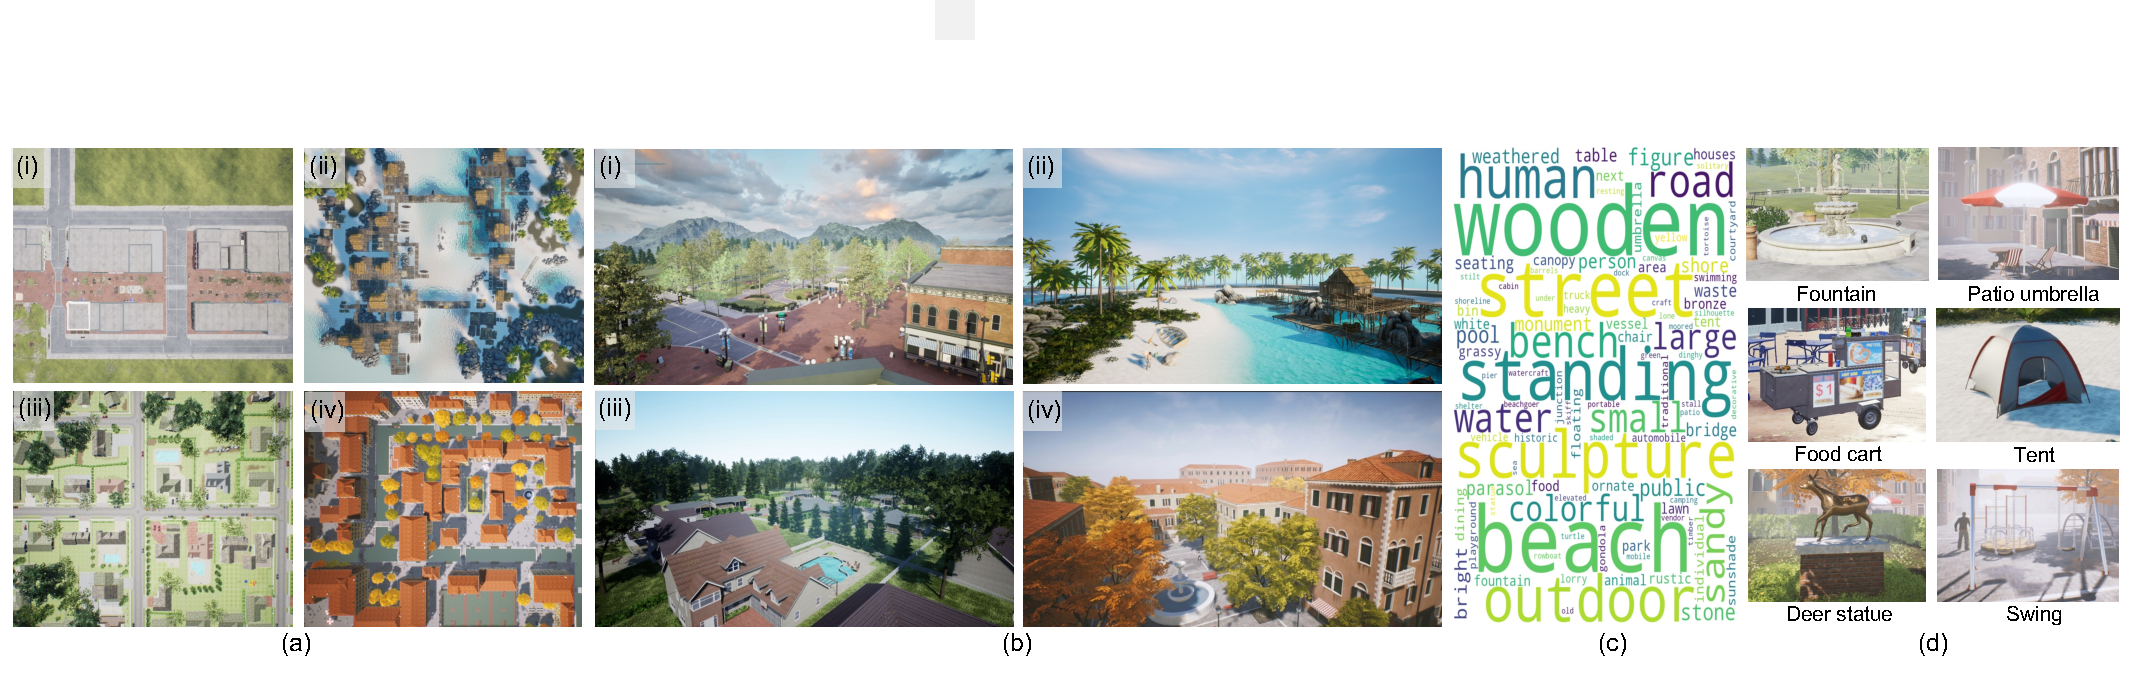
\includegraphics[width=0.99\linewidth]{figures/simenv-2.pdf}
    \caption{(a) Top-down views and (b) snapshots of four simulation environments: (i) Downtown, (ii) Cabinlake, (iii) Neighborhood, and (iv) Venice. (c) Word cloud of task instructions. (d) Images of example target objects.}
    \label{fig:simenv}
    \vspace{-12pt}
\end{figure*}

\subsection{Continuous Trajectory Refinement}\label{V-D}
During the exploration phase, once the global cluster visitation order is 
determined, we refine the local viewpoint selection across consecutive frontier clusters to minimize trajectory execution time~\cite{zhou2021fuel}. 
Upon target confirmation from the ADTR module, the system transitions to goal-directed navigation, generating a viewpoint around the verified target position with direct line-of-sight. 
Given the next viewpoint to be visited, whether in exploration or goal-directed navigation, we generate smooth, continuous B-spline trajectories that optimize both smoothness and execution time while satisfying safety and dynamic feasibility constraints~\cite{zhou2019robust}. 
The complete trajectory generation process runs in real-time, with replanning triggered whenever new frontiers are discovered or the 3D value map is updated, enabling efficient exploration in partially unknown outdoor environments.
